\begin{landscape}
\begin{figurels}
    \centering
    \caption{Systematics of the Gadolinium isotopes. $^{154}$Gd has an anomalously large connection between the first excited $0^+$ state and the ground state. The arrows shown are the B(E2) components of the transitions, in single particle Weisskopf units \citep{reich09:_nds_154,reich12:_nds_156,nica17:_nds_158,reich05:_nds_160}. The $R_{4/2}$ values beneath each nucleus are a ratio of the energies of the first excited $2^+$ and $4^+$ states, both in the ground state band. This ratio gives a rough measure of deformation.}
    \label{fig:Gd_Sys}
\end{figurels}
% \addtocounter{figure}{-1}
\begin{figurels}
    \centering
    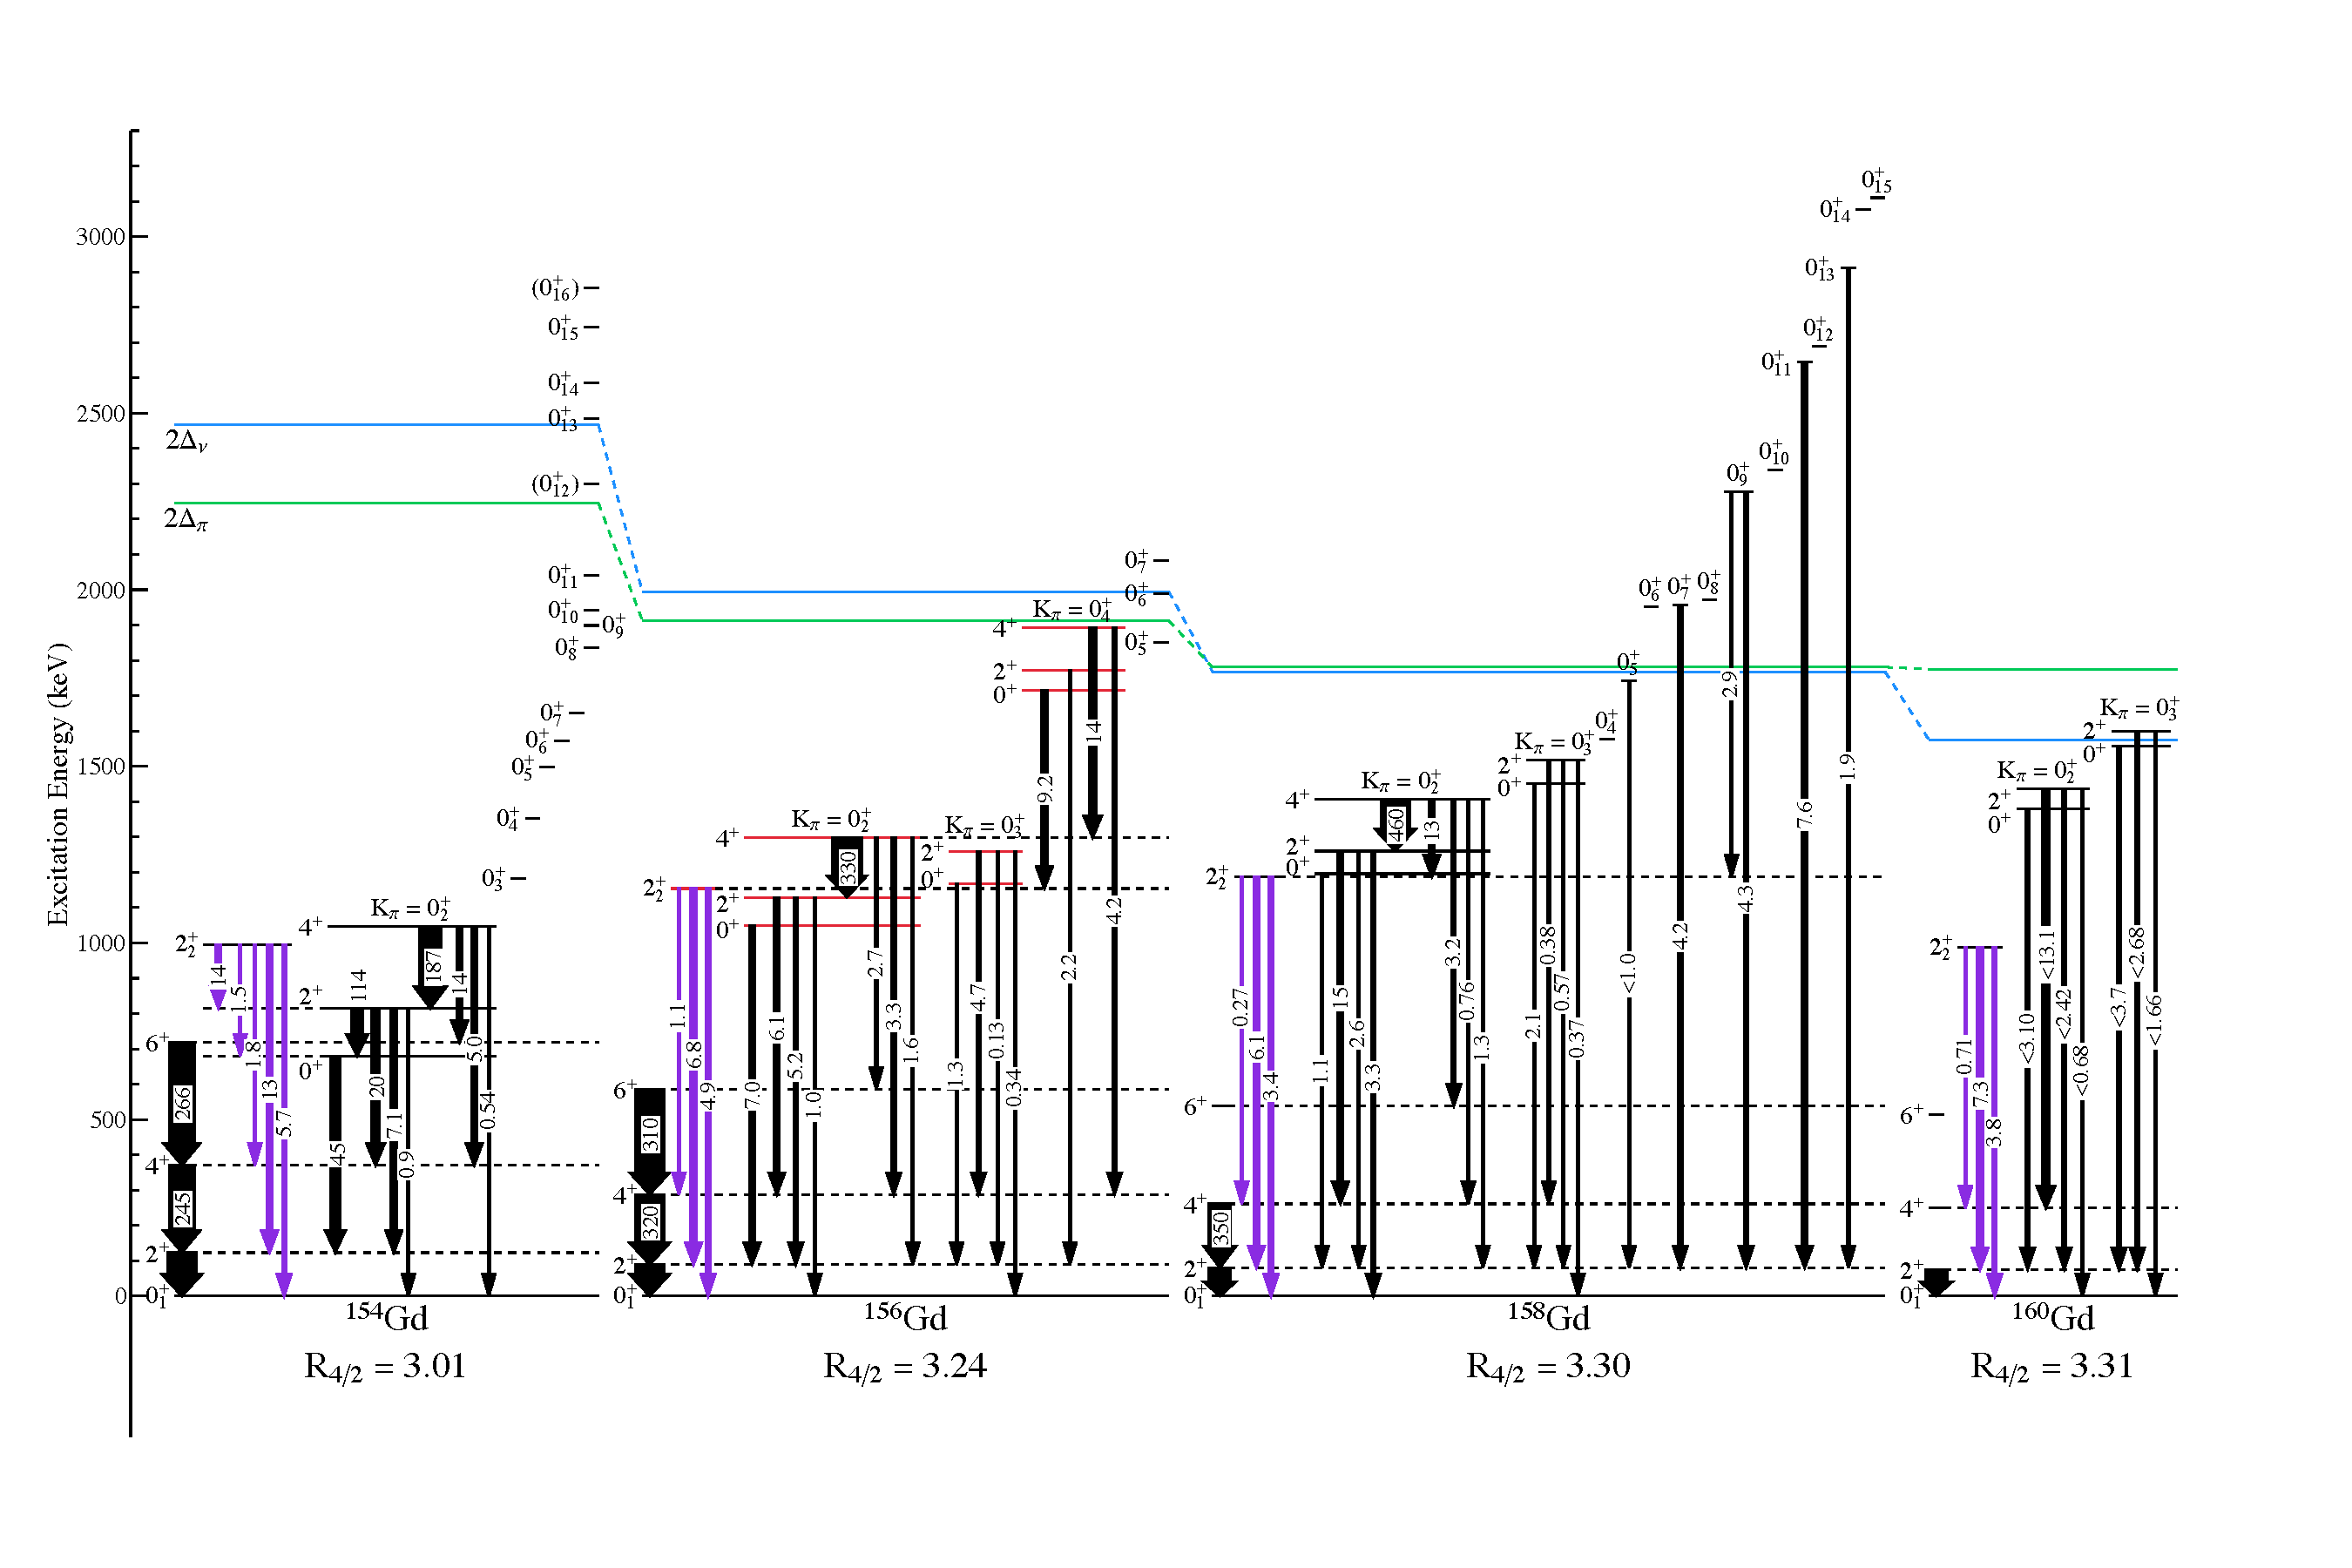
\includegraphics[width=1.35\textwidth]{154GdTablesAndFigs/Gd_Schematic_v2.pdf}
\end{figurels}
\end{landscape}